\section{Semantic matching}
\begin{itemize}
	\item \textit{Vocabulary gap}: query and document might use different lexical representation for the same entity $\implies$ resolve by semantic matching
	\item Represent query and document by their meaning, not lexical/word level
	\item This will help to identify synonyms and/or semantic relatedness for computing similarity
	\item To get such a representation, one idea is to apply dimensionality reduction. This relies on the assumption that the dimension of the data is actually lower than i.e. vocabulary size
	\item Similar data in terms of semantic will be (hopefully) similar in reduced dimensions as well
\end{itemize}
\subsection{Latent Semantic Indexing}
\begin{itemize}
	\item We represent all documents and queries in a term-document matrix:
	$$X = \left[\begin{array}{cccc}
	| & | &  & | \\
	x_1 & x_2 & \dots & x_m \\
	| & | &  & | 
	\end{array}\right]$$
	where $m$ rows represent the documents, and $n$ rows the terms. A single cell in the matrix $X$ specifies the term frequency $\text{tf}(w;d)$. Note that we would also add the queries in $X$ as documents.
	\item On this matrix, we apply Singular Value Decomposition (SVD) so that $X_{n\times m} = U_{n \times r} \Sigma_{r\times r} V_{m\times r}^T$
	\begin{itemize}
		\item $\bm{U}_{n \times r}$ represents the word/term embedding along rows (one word per row). The columns are the "semantic" dimensions that e.g. represent topics/hidden lower-dimensional space. 
		\item $\bm{V}_{m \times r}$ similarly represents the embedding of documents (one doc per row, but is transposed in calculation). 
		\item $\bm{\Sigma}_{r \times r}$ is a square, diagonal matrix. The magnitude of a singular value represents the importance of the corresponding latent dimension in the collection/data. It is always sorted from the highest value in first place to lowest value in last place.
	\end{itemize}
	\begin{figure}[ht]
		\centering
		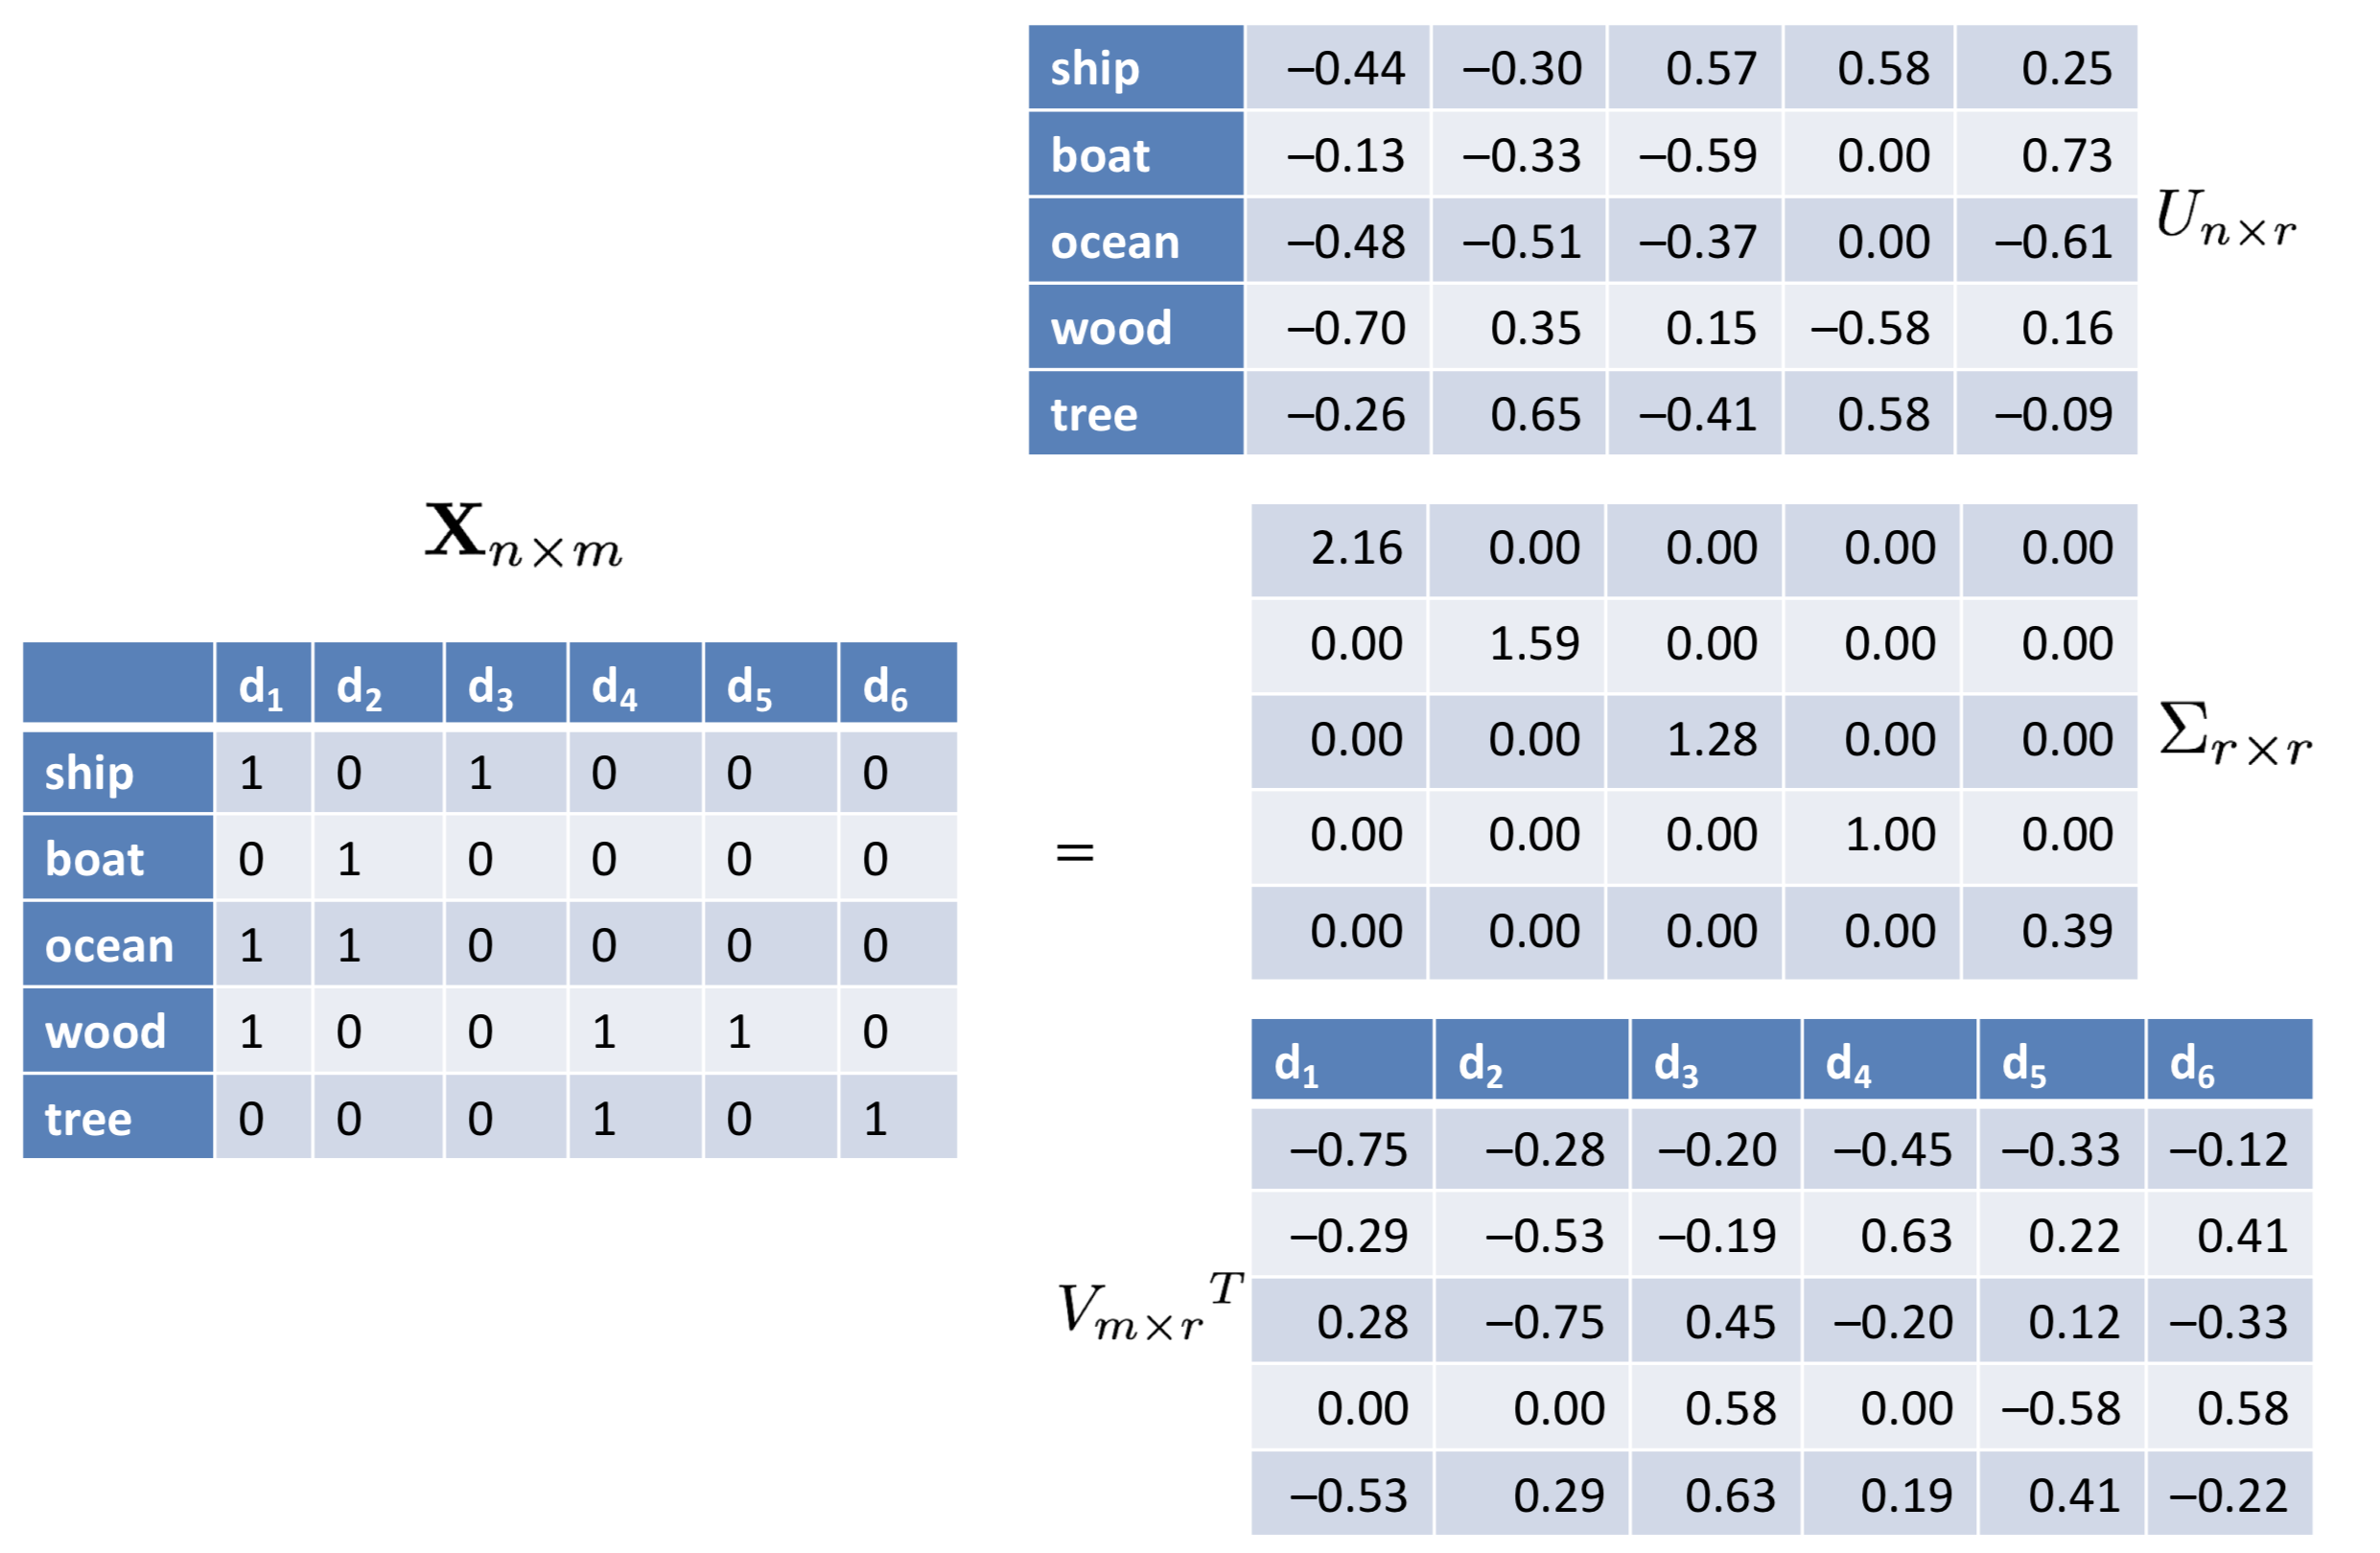
\includegraphics[width=0.5\textwidth]{figures/semantic_matching_SVD_example.png}
		\caption{Example of SVD for 6 documents and 5 terms}
		\label{img:semantic_matching_SVD_example}
	\end{figure}
	\item To reduce dimensions to $k$, we simply drop those with the lowest values in $\Sigma$. These dimensions may be noise and make things dissimilar when they actually are on topic level. $k$ is hyperparameter.
	\item In case of Figure~\ref{img:semantic_matching_SVD_example} with $k=2$, we would drop the last three dimensions. This leads to our new embeddings $X'$ for the documents. The resulting matrices would look like as in Figure~\ref{img:semantic_matching_SVD_example_2}.
	\begin{figure}[ht]
		\centering
		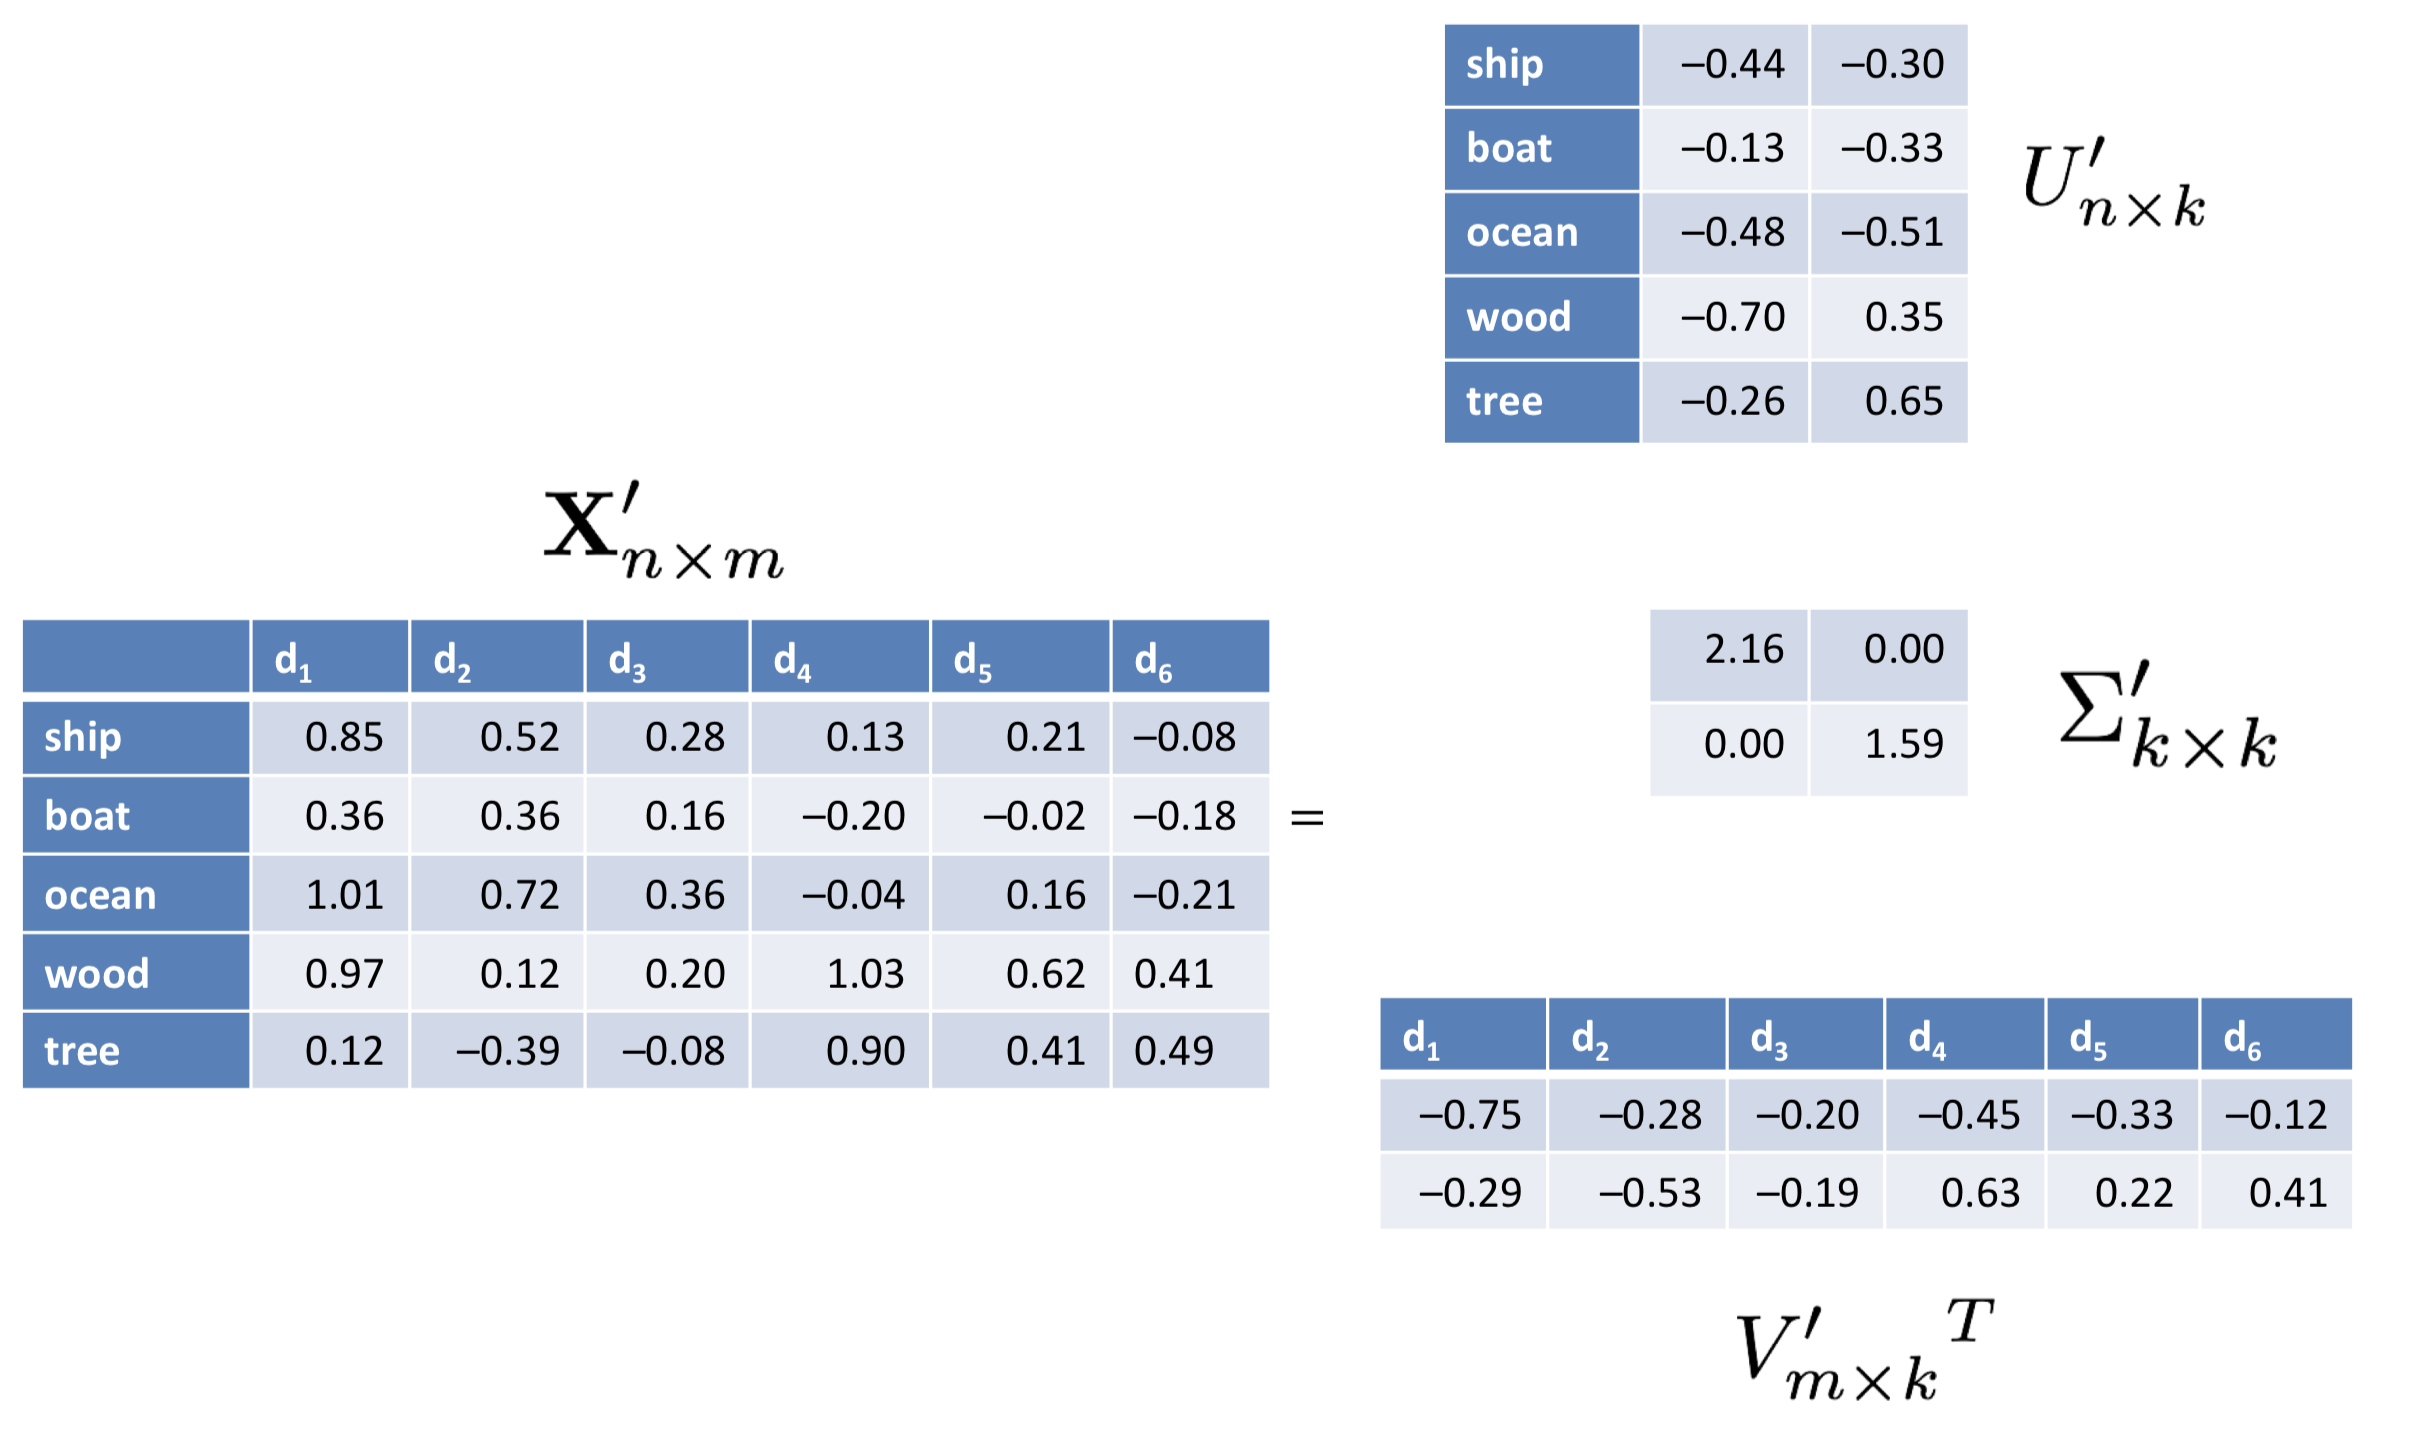
\includegraphics[width=0.5\textwidth]{figures/semantic_matching_SVD_example_2.png}
		\caption{Reduced dimensions by $k=2$ for 6 documents and 5 terms}
		\label{img:semantic_matching_SVD_example_2}
	\end{figure}
	\item The similarity between documents/queries can be calculated by cosine similarity (dot product) between their new embeddings in $X'$. Furthermore, we can also compute the similarity between terms by using the rows.
	\item Choice of $k$:
	\begin{itemize}
		\item The choice of $k$ is critical in IR. The ideal value of $k$ would be large enough to fit all the real structure in the data, but small enough to compress/group terms together that are very similar (less noise).
		\item Typically, different values of $k$ are tested and compared by their performance. For example, a high precision but low recall suggests a poor generalization of the model. Therefore, we should decrease $k$ in this case.
	\end{itemize}
	\item LSI addresses synonymy by mapping similar words in the same dimensions. The cost of such a mapping is lower than for unrelated words as they occur similar/same documents. 
	\item \textbf{Strengths} of LSI
	\begin{itemize}
		\item Using $X'$ instead of $X$ show performance increase as we filter out the noise
		\item $X'$ represents the best approximation of $X$ with a matrix of rank $k$: $X' = \argmin\limits_{X':\text{rank}(X')=k} ||X-X'||$
		\item Is mostly combined with lexical methods like BM25 to not lose "obvious" matches
	\end{itemize}
	\item \textbf{Weaknesses} of LSI
	\begin{itemize}
		\item A huge storage is required as the matrices $U$ and $V$ are dense (less zeros)
		\item Representations are not interpretable, and it is not guaranteed that hidden dimensions represent topics
		\item $k$ is often not easy to determine and requires multiple tests
		\item SVD assumes orthogonal dimensions on which the variance is maximum which is not always the case
		\item The model is not generative or probabilistic, which makes it hard to extend collection by new documents/queries (worst case: redo whole SVD)
	\end{itemize}
	\item One alternative is Non-negative Matrix Factorization which leads to smaller, positive matrices (but doesn't solve the other problems)
\end{itemize}
\subsection{Probabilistic Latent Semantic Indexing}
\begin{itemize}
	\item (Pseudo-)generative model with which we try to detect key topics in the collection in an unsupervised fashion. The model describes how we would generate docs for certain topics
	\item Every topic has its own language model/distribution over words in vocabulary in a unigram/bag-of-word style: $p(w|z=1), p(w|z=2),...$ where $z$ is the variable representing the topics. 
	\item A document is represented by the distribution of these topics in the document. Generating a document would require to first sample a topic based on the topic distribution of the document, and then generating a word based on the language model of the topic. The order of the words is not taken into account. An example is shown in Figure~\ref{img:semantic_matching_PLSI_example}.
	\begin{figure}[ht]
		\centering
		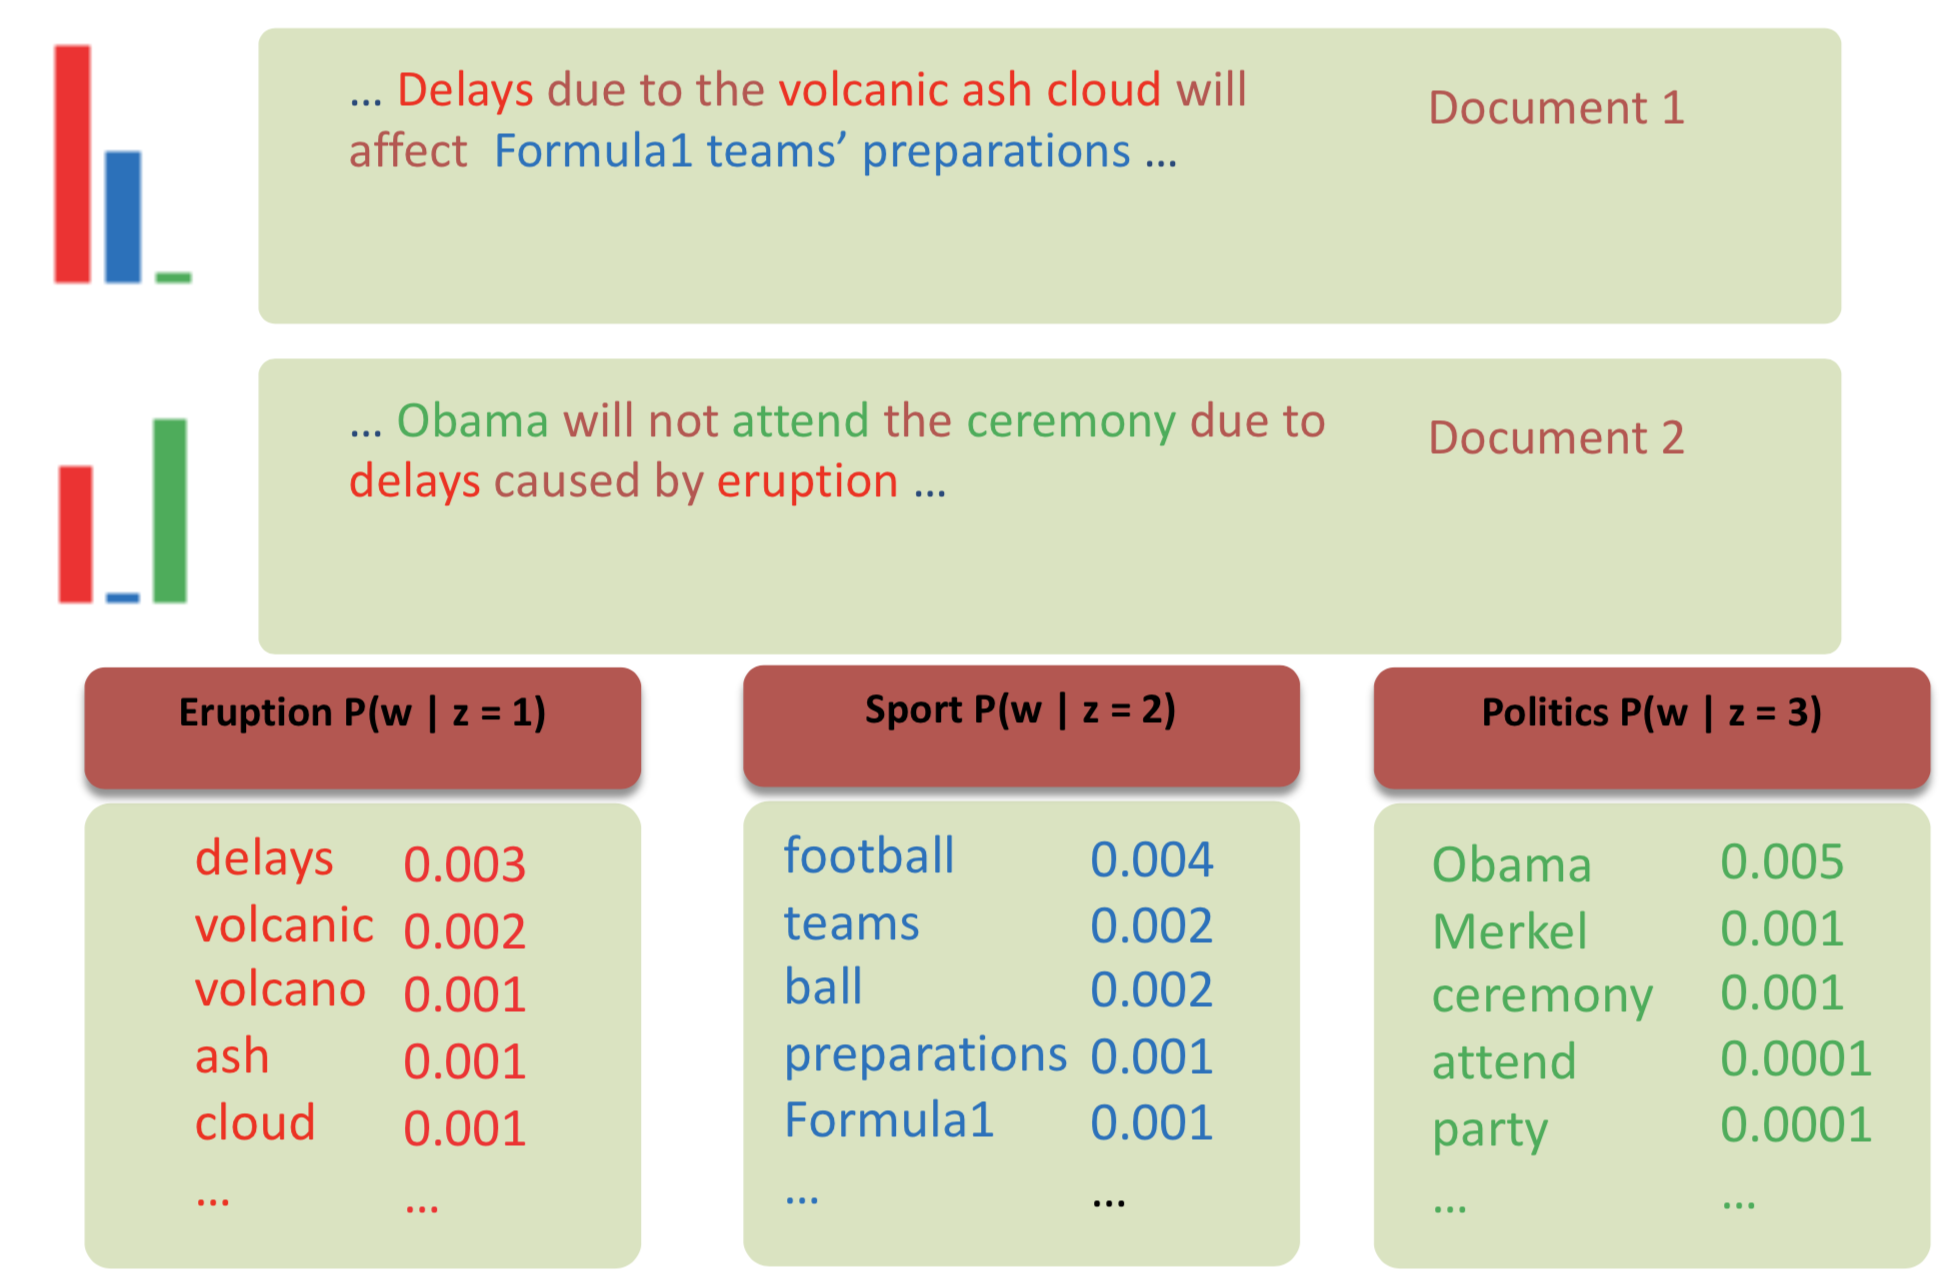
\includegraphics[width=0.5\textwidth]{figures/semantic_matching_PLSI_example.png}
		\caption{Example of document representation in PLSI}
		\label{img:semantic_matching_PLSI_example}
	\end{figure}
	\item For semantic matching, we calculate the cosine similarity between the topic distributions of the query and the document.
	\item PSLA can have problems with stop words (common words that occur in every document frequently like "the" or "and"). To prevent that, we summarize all stop words in a separate background topic model which is equally shared by all docs. Before generating a word, we toss a biased coin to decide whether to retrieve a word from the background or standard topic model. Note that in matching, these stop words are masked out by that
\end{itemize}
\subsubsection{Retrieving distributions}
\begin{itemize}
	\item Input: collection of $N$ documents, number of topics $K$
	\item Output:
	\begin{itemize}
		\item Distributions over words $\phi_{(z,w)} = p(w|z)$ for $z\in \left\{1,...,K\right\}$ with $\sum_{w\in V} p(w|z) = 1$
		\item Distributions over topics in all documents: $\theta_{d,z} = p(z|d)$ for every $d$, with $\sum_{z=1}^{K} p(z|d) = 1$
	\end{itemize} 
	\item We try to solve problem by MLE. The probability of $w$ appearing at position $i$ in the document $d$ is:
	$$p(d_i = w | \Phi, \theta_d) = \sum\limits_{z=1}^{K} \phi_{(z,w)} \theta_{d,z}$$
	The joint likelihood of the entire dataset is:
	$$p(W|\Phi, \Theta) = \prod\limits_{d\in D}\prod\limits_{w\in V}\left(\sum\limits_{z=1}^{K} \phi_{(z,w)} \theta_{d,z}\right)^{\text{tf}(w;d)} $$
	\item Taking the two constraints into account, we get an optimization problem which we can solve by the EM algorithm. For that, we assume that we know from which topic a word was generated at position $i$ in the document by $R_{d_i}$:
	$$p(W|R,\Phi,\Theta) = \prod\limits_{d\in D}\prod\limits_{i=1}^{N_i}\sum\limits_{z=1}^{K} R_{(d_i,z)} \left(\phi_{(z,w)} \theta_{d,z}\right)$$
	\item For the EM algorithm, we would update $R_{d_i}$ during the expectation step by $R_{d_i} = \frac{\phi_{(z,w_i)\theta_{(d,z)}}}{\sum_{z=1}^{K} \phi_{(z,w_i)\theta_{(d,z)}}}$. The maximization step consists of updating $\Theta$ and $\Phi$: $\theta_{(d,z)} = \frac{\sum_{d_i} R_{(d_i,z)}}{|d|}$, $\phi_{(z,w)} = \frac{\sum_{d \in D} n(d,w) R_{(w,z)}}{\sum_{w' \in V} \sum_{d \in D} n(d,w')R_{(w',z)}}$
	\item PLSA is able to learn topics with their corresponding word distributions. However, there are still some drawbacks:
	\begin{itemize}
		\item It is still not a fully generative model. After running PSLA, we have topic distribution for documents we initially had, but we cannot extend it to new documents (or only hardly with heuristics)
		\item Prone to overfitting
	\end{itemize}
\end{itemize}
\subsubsection{Latent Dirichlet Allocation (LDA)}
\begin{itemize}
	\item Takes PLSA but makes it a generative model with Dirichlet prior. Can also be seen as a Bayesian treatment of PLSA
	\item Instead of probabilities for every document, we now simply define two hyperparameters $\alpha$ and $\beta$
	\item For every topic $z=1,...,K$, we draw a word distribution $\phi_z \sim \text{Dir}(\beta)$. Thus, $\beta$ determines how words are distributed per topic
	\item For each document $d$, we sample a topic distribution $\theta_d \sim \text{Dir}(\alpha)$. The alpha therefore controls the mixture of topics for any given document.
	\item The words in the documents are then sampled by the probabilities $\phi_z$ and $\theta_d$. Note that this is a fully generative model as we can generate as many new documents as we need.
\end{itemize}
\subsubsection{Graphical Models and Probabilistic Topic Models}
\begin{itemize}
	\item We can represent every probabilistic topic model as graphical model which abstracts the conditional independence relationships
	\item For example, Figure~\ref{img:semantic_matching_graphical_models_LDA} visualizes the graphical model of the Latent Dirichlet Allocation
	\begin{figure}[ht]
		\centering
		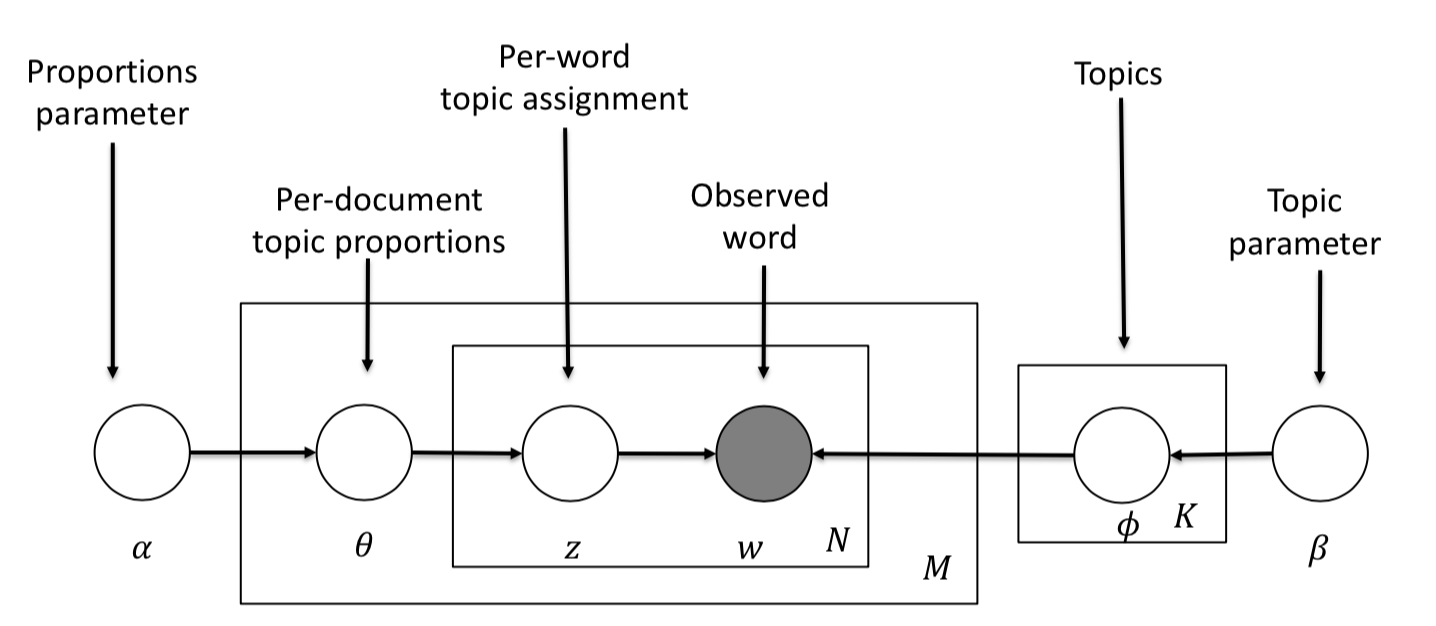
\includegraphics[width=0.5\textwidth]{figures/semantic_matching_graphical_models_LDA.png}
		\caption{Graphical model of LDA}
		\label{img:semantic_matching_graphical_models_LDA}
	\end{figure}
	\item In this diagrams, it is easier to show extensions. For instance, Figure~\ref{img:semantic_matching_graphical_models_author_model} visualizes the Author-Topic model where we add an observed variable of the author of a document. This observation affects the probability distributions over words for each topic in a document 
	\begin{figure}[ht]
		\centering
		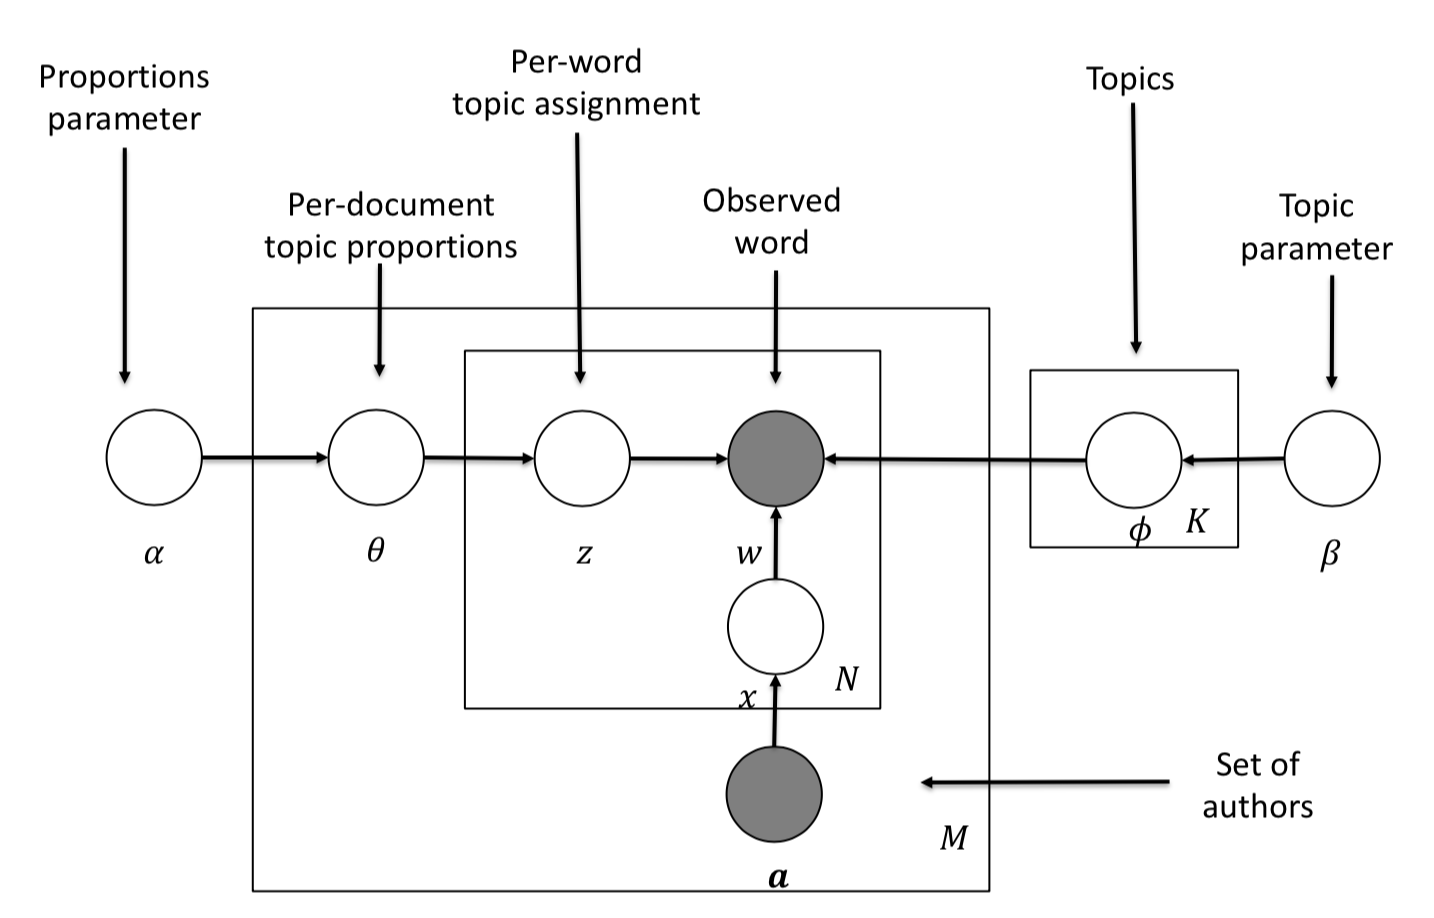
\includegraphics[width=0.5\textwidth]{figures/semantic_matching_graphical_models_author_model.png}
		\caption{Graphical model of the Author-topic model}
		\label{img:semantic_matching_graphical_models_author_model}
	\end{figure}
	% semantic_matching_graphical_models_author_model.png
\end{itemize}
\subsection{Probabilistic Topic Models in IR}
\begin{enumerate}
	\item \textbf{Topic matching}
	\begin{itemize}
		\item Represent document by $p(z|d)$ and query by $p(z|q)$
		\item Take the KL divergence or similar measure to find score/similarity between the distributions
		\item But: query is very short so that topic model is harder to infer without having too much noise
	\end{itemize}
	\item \textbf{Smoothing}
	\begin{itemize}
		\item Smooth probabilities according to the topics in the document:
		\begin{equation*}
			\begin{split}
				p(w|d) & = \lambda p_{\mu}(w|d) + (1 - \lambda) p_{\text{tm}}(w|d)\\
				& = \lambda p_{\mu}(w|d) + (1 - \lambda) \left(\sum\limits_{z=1}^{K} p(w|z) p(z|d)\right)
			\end{split}
		\end{equation*}
		\item Thus we apply Jelinek-Mercer smoothing where the context is replaced by the topic word distributions of the document
	\end{itemize}
	\item \textbf{Query expansion}
	\begin{itemize}
		\item We can build an own language model for a given query by using the word distributions of the topics:
		$$p_{\text{tm}}(w|q) = \sum\limits_{z=1}^{K} p(w|z) p(z|q)$$
	\end{itemize}
\end{enumerate}